\begin{frame}
  \frametitle{Results for the Previous Week}

  \begin{center}
    Here are the results for last week:

    \bigskip
    
    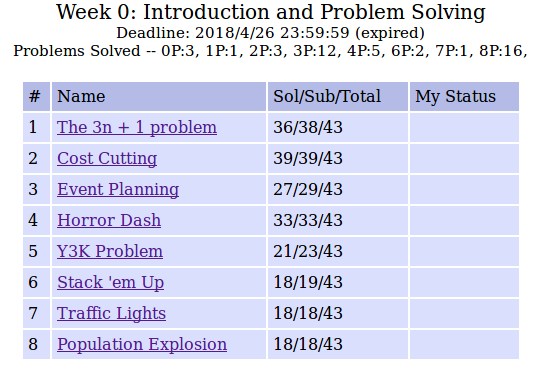
\includegraphics[width=0.8\textwidth]{img/resultW0}
    
    \bigskip

    Hope you enjoyed the warm up!
  \end{center}

\end{frame}

\begin{frame}[fragile]
  \frametitle{Comments from e-mails and questions -- 1}

  \begin{block}{Submission with Java}
    Two students had \structure{``runtime error''} with Java last week
    -- don't forget that your start class MUST be called {\bf Main}.
  \end{block}

  \vfill

\begin{verbatim}
class Main {
  public static void main(String[] args) {

    // do something...

  }
}
\end{verbatim}
\end{frame}

\begin{frame}
  \frametitle{Comments from e-mails and questions -- 2}
  \begin{block}{Input/Output}
    Two other students had problems because their program printed ``Please enter a number''.

    \bigskip

    You are very kind, but please {\bf follow the specifications} strictly!
  \end{block}
  
  \vfill

  \begin{block}{Format for MANABA submission}
    One student asked if the code for MANABA had to be the same as the code for UVA.

    \bigskip

    Yes. The code you submit on MANABA must be {\bf exactly the same}
    as the code you submitted for UVA.
  \end{block}
\end{frame}

\begin{frame}
  \frametitle{Short comments about the problems:}
  \begin{itemize}
  \item Cost Cutting, Event Planning, Horror Dash -- Easiest problems (find mean, find min, find min);
    \bigskip

  \item 3n+1 -- Still easy, but a few traps -- example of {\bf Memoization};
    \bigskip

  \item Y3K Problem -- Still easy, but skip year can be a bit troublesome.
    
  \end{itemize}
\end{frame}

%\begin{frame}
%  \frametitle{Comments about the problems}
%\end{frame}
